\documentclass[twoside]{book}

% Packages required by doxygen
\usepackage{fixltx2e}
\usepackage{calc}
\usepackage{doxygen}
\usepackage{graphicx}
\usepackage[utf8]{inputenc}
\usepackage{makeidx}
\usepackage{multicol}
\usepackage{multirow}
\PassOptionsToPackage{warn}{textcomp}
\usepackage{textcomp}
\usepackage[nointegrals]{wasysym}
\usepackage[table]{xcolor}

% Font selection
\usepackage[T1]{fontenc}
\usepackage{mathptmx}
\usepackage[scaled=.90]{helvet}
\usepackage{courier}
\usepackage{amssymb}
\usepackage{sectsty}
\renewcommand{\familydefault}{\sfdefault}
\allsectionsfont{%
  \fontseries{bc}\selectfont%
  \color{darkgray}%
}
\renewcommand{\DoxyLabelFont}{%
  \fontseries{bc}\selectfont%
  \color{darkgray}%
}
\newcommand{\+}{\discretionary{\mbox{\scriptsize$\hookleftarrow$}}{}{}}

% Page & text layout
\usepackage{geometry}
\geometry{%
  a4paper,%
  top=2.5cm,%
  bottom=2.5cm,%
  left=2.5cm,%
  right=2.5cm%
}
\tolerance=750
\hfuzz=15pt
\hbadness=750
\setlength{\emergencystretch}{15pt}
\setlength{\parindent}{0cm}
\setlength{\parskip}{0.2cm}
\makeatletter
\renewcommand{\paragraph}{%
  \@startsection{paragraph}{4}{0ex}{-1.0ex}{1.0ex}{%
    \normalfont\normalsize\bfseries\SS@parafont%
  }%
}
\renewcommand{\subparagraph}{%
  \@startsection{subparagraph}{5}{0ex}{-1.0ex}{1.0ex}{%
    \normalfont\normalsize\bfseries\SS@subparafont%
  }%
}
\makeatother

% Headers & footers
\usepackage{fancyhdr}
\pagestyle{fancyplain}
\fancyhead[LE]{\fancyplain{}{\bfseries\thepage}}
\fancyhead[CE]{\fancyplain{}{}}
\fancyhead[RE]{\fancyplain{}{\bfseries\leftmark}}
\fancyhead[LO]{\fancyplain{}{\bfseries\rightmark}}
\fancyhead[CO]{\fancyplain{}{}}
\fancyhead[RO]{\fancyplain{}{\bfseries\thepage}}
\fancyfoot[LE]{\fancyplain{}{}}
\fancyfoot[CE]{\fancyplain{}{}}
\fancyfoot[RE]{\fancyplain{}{\bfseries\scriptsize Generated on Mon Jul 7 2014 14\+:26\+:30 for “\+I\+K\+Jayma” by Doxygen }}
\fancyfoot[LO]{\fancyplain{}{\bfseries\scriptsize Generated on Mon Jul 7 2014 14\+:26\+:30 for “\+I\+K\+Jayma” by Doxygen }}
\fancyfoot[CO]{\fancyplain{}{}}
\fancyfoot[RO]{\fancyplain{}{}}
\renewcommand{\footrulewidth}{0.4pt}
\renewcommand{\chaptermark}[1]{%
  \markboth{#1}{}%
}
\renewcommand{\sectionmark}[1]{%
  \markright{\thesection\ #1}%
}

% Indices & bibliography
\usepackage{natbib}
\usepackage[titles]{tocloft}
\setcounter{tocdepth}{3}
\setcounter{secnumdepth}{5}
\makeindex

% Hyperlinks (required, but should be loaded last)
\usepackage{ifpdf}
\ifpdf
  \usepackage[pdftex,pagebackref=true]{hyperref}
\else
  \usepackage[ps2pdf,pagebackref=true]{hyperref}
\fi
\hypersetup{%
  colorlinks=true,%
  linkcolor=blue,%
  citecolor=blue,%
  unicode%
}

% Custom commands
\newcommand{\clearemptydoublepage}{%
  \newpage{\pagestyle{empty}\cleardoublepage}%
}


%===== C O N T E N T S =====

\begin{document}

% Titlepage & ToC
\hypersetup{pageanchor=false,
             bookmarks=true,
             bookmarksnumbered=true,
             pdfencoding=unicode
            }
\pagenumbering{roman}
\begin{titlepage}
\vspace*{7cm}
\begin{center}%
{\Large “\+I\+K\+Jayma” }\\
\vspace*{1cm}
{\large Generated by Doxygen 1.8.7}\\
\vspace*{0.5cm}
{\small Mon Jul 7 2014 14:26:30}\\
\end{center}
\end{titlepage}
\clearemptydoublepage
\tableofcontents
\clearemptydoublepage
\pagenumbering{arabic}
\hypersetup{pageanchor=true}

%--- Begin generated contents ---
\chapter{Hierarchical Index}
\section{Class Hierarchy}
This inheritance list is sorted roughly, but not completely, alphabetically\+:\begin{DoxyCompactList}
\item N\+S\+Error\begin{DoxyCompactList}
\item \contentsline{section}{I\+J\+Error}{\pageref{interface_i_j_error}}{}
\end{DoxyCompactList}
\item N\+S\+Object\begin{DoxyCompactList}
\item \contentsline{section}{I\+J\+Abstract\+Document}{\pageref{interface_i_j_abstract_document}}{}
\item \contentsline{section}{I\+J\+Abstract\+Repository}{\pageref{interface_i_j_abstract_repository}}{}
\item \contentsline{section}{I\+J\+A\+F\+Networking\+Backend}{\pageref{interface_i_j_a_f_networking_backend}}{}
\end{DoxyCompactList}
\end{DoxyCompactList}

\chapter{Class Index}
\section{Class List}
Here are the classes, structs, unions and interfaces with brief descriptions\+:\begin{DoxyCompactList}
\item\contentsline{section}{\hyperlink{interface_i_j_abstract_document}{I\+J\+Abstract\+Document} }{\pageref{interface_i_j_abstract_document}}{}
\item\contentsline{section}{\hyperlink{interface_i_j_abstract_repository}{I\+J\+Abstract\+Repository} }{\pageref{interface_i_j_abstract_repository}}{}
\item\contentsline{section}{\hyperlink{interface_i_j_a_f_networking_backend}{I\+J\+A\+F\+Networking\+Backend} }{\pageref{interface_i_j_a_f_networking_backend}}{}
\item\contentsline{section}{\hyperlink{interface_i_j_error}{I\+J\+Error} }{\pageref{interface_i_j_error}}{}
\end{DoxyCompactList}

\chapter{File Index}
\section{File List}
Here is a list of all files with brief descriptions\+:\begin{DoxyCompactList}
\item\contentsline{section}{I\+K\+Jayma/\hyperlink{_i_j_abstract_document_8h}{I\+J\+Abstract\+Document.\+h} }{\pageref{_i_j_abstract_document_8h}}{}
\item\contentsline{section}{I\+K\+Jayma/\hyperlink{_i_j_abstract_repository_8h}{I\+J\+Abstract\+Repository.\+h} }{\pageref{_i_j_abstract_repository_8h}}{}
\item\contentsline{section}{I\+K\+Jayma/\hyperlink{_i_j_a_f_networking_backend_8h}{I\+J\+A\+F\+Networking\+Backend.\+h} }{\pageref{_i_j_a_f_networking_backend_8h}}{}
\item\contentsline{section}{I\+K\+Jayma/\hyperlink{_i_j_error_8h}{I\+J\+Error.\+h} }{\pageref{_i_j_error_8h}}{}
\end{DoxyCompactList}

\chapter{Class Documentation}
\hypertarget{interface_i_j_abstract_document}{\section{I\+J\+Abstract\+Document Class Reference}
\label{interface_i_j_abstract_document}\index{I\+J\+Abstract\+Document@{I\+J\+Abstract\+Document}}
}


{\ttfamily \#import $<$I\+J\+Abstract\+Document.\+h$>$}

Inheritance diagram for I\+J\+Abstract\+Document\+:\begin{figure}[H]
\begin{center}
\leavevmode
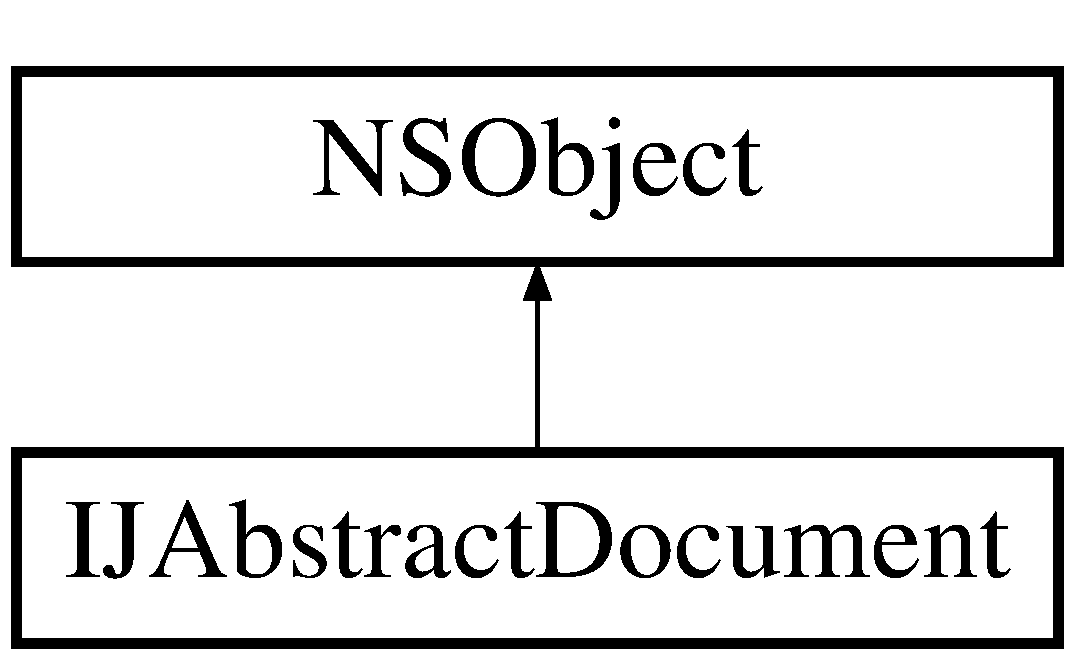
\includegraphics[height=2.000000cm]{interface_i_j_abstract_document}
\end{center}
\end{figure}
\subsection*{Instance Methods}
\begin{DoxyCompactItemize}
\item 
(id) -\/ \hyperlink{interface_i_j_abstract_document_a54f32ec1d0b54e699038c442c9a3e165}{init\+With\+Dictionary\+:}
\begin{DoxyCompactList}\small\item\em A\+B\+S\+T\+R\+A\+C\+T M\+E\+T\+H\+O\+D. You'll need to write your custom implementation. \end{DoxyCompactList}\item 
(void) -\/ \hyperlink{interface_i_j_abstract_document_a2be2916d90a20828bc0b1ca3947d7ca9}{refresh\+With\+Dictionary\+:}
\begin{DoxyCompactList}\small\item\em A\+B\+S\+T\+R\+A\+C\+T M\+E\+T\+H\+O\+D. You'll need to write your custom implementation. \end{DoxyCompactList}\item 
(N\+S\+Dictionary $\ast$) -\/ \hyperlink{interface_i_j_abstract_document_a0e928e60fba0d581ca2071771fa57ce6}{dictionary\+Representation}
\begin{DoxyCompactList}\small\item\em A\+B\+S\+T\+R\+A\+C\+T M\+E\+T\+H\+O\+D. You'll need to write your custom implementation. \end{DoxyCompactList}\end{DoxyCompactItemize}
\subsection*{Properties}
\begin{DoxyCompactItemize}
\item 
N\+S\+String $\ast$ \hyperlink{interface_i_j_abstract_document_aa2696bc058879761be4214d033e54870}{document\+Id}
\end{DoxyCompactItemize}


\subsection{Method Documentation}
\hypertarget{interface_i_j_abstract_document_a0e928e60fba0d581ca2071771fa57ce6}{\index{I\+J\+Abstract\+Document@{I\+J\+Abstract\+Document}!dictionary\+Representation@{dictionary\+Representation}}
\index{dictionary\+Representation@{dictionary\+Representation}!I\+J\+Abstract\+Document@{I\+J\+Abstract\+Document}}
\subsubsection[{dictionary\+Representation}]{\setlength{\rightskip}{0pt plus 5cm}-\/ (N\+S\+Dictionary $\ast$) dictionary\+Representation 
\begin{DoxyParamCaption}
{}
\end{DoxyParamCaption}
}}\label{interface_i_j_abstract_document_a0e928e60fba0d581ca2071771fa57ce6}


A\+B\+S\+T\+R\+A\+C\+T M\+E\+T\+H\+O\+D. You'll need to write your custom implementation. 

Retrieve a dictionary representation of the Abstract\+Document. \hypertarget{interface_i_j_abstract_document_a54f32ec1d0b54e699038c442c9a3e165}{\index{I\+J\+Abstract\+Document@{I\+J\+Abstract\+Document}!init\+With\+Dictionary\+:@{init\+With\+Dictionary\+:}}
\index{init\+With\+Dictionary\+:@{init\+With\+Dictionary\+:}!I\+J\+Abstract\+Document@{I\+J\+Abstract\+Document}}
\subsubsection[{init\+With\+Dictionary\+:}]{\setlength{\rightskip}{0pt plus 5cm}-\/ (id) init\+With\+Dictionary\+: 
\begin{DoxyParamCaption}
\item[{(N\+S\+Dictionary $\ast$)}]{dictionary}
\end{DoxyParamCaption}
}}\label{interface_i_j_abstract_document_a54f32ec1d0b54e699038c442c9a3e165}


A\+B\+S\+T\+R\+A\+C\+T M\+E\+T\+H\+O\+D. You'll need to write your custom implementation. 

Init an Abstract\+Document with a dictionary. \hypertarget{interface_i_j_abstract_document_a2be2916d90a20828bc0b1ca3947d7ca9}{\index{I\+J\+Abstract\+Document@{I\+J\+Abstract\+Document}!refresh\+With\+Dictionary\+:@{refresh\+With\+Dictionary\+:}}
\index{refresh\+With\+Dictionary\+:@{refresh\+With\+Dictionary\+:}!I\+J\+Abstract\+Document@{I\+J\+Abstract\+Document}}
\subsubsection[{refresh\+With\+Dictionary\+:}]{\setlength{\rightskip}{0pt plus 5cm}-\/ (void) refresh\+With\+Dictionary\+: 
\begin{DoxyParamCaption}
\item[{(N\+S\+Dictionary $\ast$)}]{dictionary}
\end{DoxyParamCaption}
}}\label{interface_i_j_abstract_document_a2be2916d90a20828bc0b1ca3947d7ca9}


A\+B\+S\+T\+R\+A\+C\+T M\+E\+T\+H\+O\+D. You'll need to write your custom implementation. 

Refresh the Abstract\+Document with a dictionary. 

\subsection{Property Documentation}
\hypertarget{interface_i_j_abstract_document_aa2696bc058879761be4214d033e54870}{\index{I\+J\+Abstract\+Document@{I\+J\+Abstract\+Document}!document\+Id@{document\+Id}}
\index{document\+Id@{document\+Id}!I\+J\+Abstract\+Document@{I\+J\+Abstract\+Document}}
\subsubsection[{document\+Id}]{\setlength{\rightskip}{0pt plus 5cm}-\/ (N\+S\+String$\ast$) document\+Id\hspace{0.3cm}{\ttfamily [read]}, {\ttfamily [write]}, {\ttfamily [nonatomic]}, {\ttfamily [strong]}}}\label{interface_i_j_abstract_document_aa2696bc058879761be4214d033e54870}
The document\+Id used in the server calls. This propery has to exist and have a valid value. 

The documentation for this class was generated from the following file\+:\begin{DoxyCompactItemize}
\item 
I\+K\+Jayma/\hyperlink{_i_j_abstract_document_8h}{I\+J\+Abstract\+Document.\+h}\end{DoxyCompactItemize}

\hypertarget{interface_i_j_abstract_repository}{\section{I\+J\+Abstract\+Repository Class Reference}
\label{interface_i_j_abstract_repository}\index{I\+J\+Abstract\+Repository@{I\+J\+Abstract\+Repository}}
}


{\ttfamily \#import $<$I\+J\+Abstract\+Repository.\+h$>$}

Inheritance diagram for I\+J\+Abstract\+Repository\+:\begin{figure}[H]
\begin{center}
\leavevmode
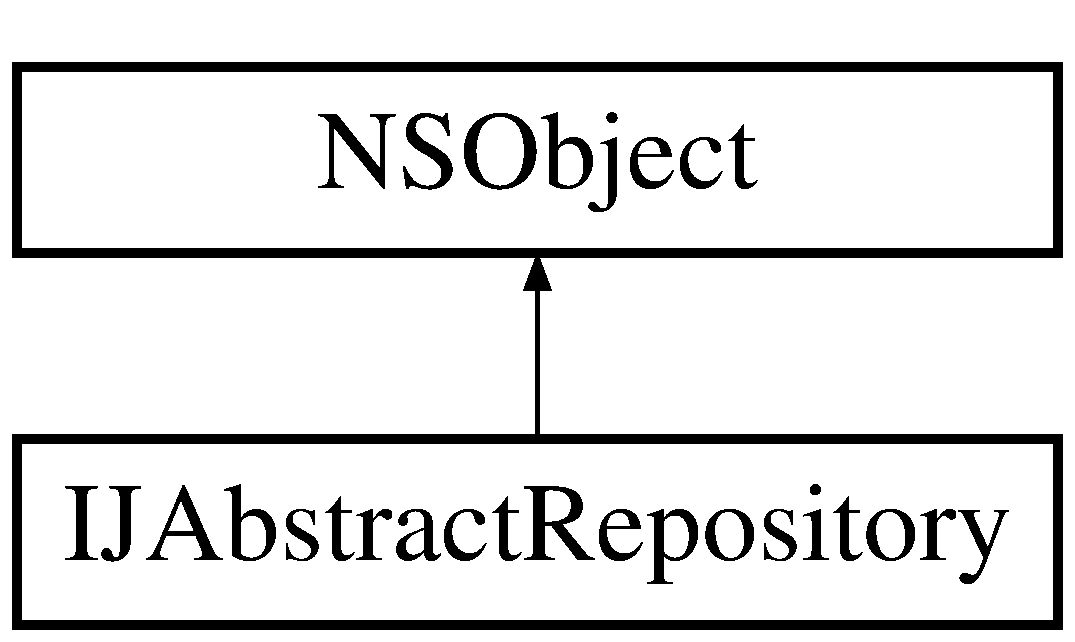
\includegraphics[height=2.000000cm]{interface_i_j_abstract_repository}
\end{center}
\end{figure}
\subsection*{Instance Methods}
\begin{DoxyCompactItemize}
\item 
(id) -\/ \hyperlink{interface_i_j_abstract_repository_aaf55a25070c26c7c4a196fd351d26120}{init\+With\+Backend\+:}
\begin{DoxyCompactList}\small\item\em A\+B\+S\+T\+R\+A\+C\+T M\+E\+T\+H\+O\+D. You'll need to write your custom implementation. \end{DoxyCompactList}\item 
(void) -\/ \hyperlink{interface_i_j_abstract_repository_afc684685531c52dc0416f3102e36b863}{create\+Document\+:success\+:failure\+:}
\begin{DoxyCompactList}\small\item\em Create a document in the server. \end{DoxyCompactList}\item 
(void) -\/ \hyperlink{interface_i_j_abstract_repository_a2f12e0f9ef13c70b111a0a62380e5057}{update\+Document\+:success\+:failure\+:}
\begin{DoxyCompactList}\small\item\em Update a document in the server. \end{DoxyCompactList}\item 
(void) -\/ \hyperlink{interface_i_j_abstract_repository_a4775f90e1f9bea0059570e333d63f627}{delete\+Document\+:success\+:failure\+:}
\begin{DoxyCompactList}\small\item\em Delete a document in the server. \end{DoxyCompactList}\item 
(void) -\/ \hyperlink{interface_i_j_abstract_repository_abe7d6b453fb5a147da1a5aff76aac81c}{delete\+Document\+With\+Id\+:success\+:failure\+:}
\begin{DoxyCompactList}\small\item\em Delete a document in the server. \end{DoxyCompactList}\item 
(void) -\/ \hyperlink{interface_i_j_abstract_repository_a66ba7a11b374ddb499bb7da97cd27151}{find\+Document\+With\+Id\+:success\+:failure\+:}
\begin{DoxyCompactList}\small\item\em Find a document in the server. \end{DoxyCompactList}\item 
(void) -\/ \hyperlink{interface_i_j_abstract_repository_a892ede1f469ee2112a67c79e6139071f}{find\+Documents\+With\+Conditions\+:success\+:failure\+:}
\begin{DoxyCompactList}\small\item\em Find a list of documents in the server. \end{DoxyCompactList}\item 
(void) -\/ \hyperlink{interface_i_j_abstract_repository_a719a18f043952f383d27a9d62e0c8ace}{find\+All\+Documents\+With\+Success\+:failure\+:}
\begin{DoxyCompactList}\small\item\em Find all documents in the server. \end{DoxyCompactList}\item 
(void) -\/ \hyperlink{interface_i_j_abstract_repository_a1235a257e5e040cb665ad9607b9a8e42}{refresh\+Document\+:success\+:failure\+:}
\begin{DoxyCompactList}\small\item\em Refresh a local document. \end{DoxyCompactList}\item 
(\hyperlink{interface_i_j_abstract_document}{I\+J\+Abstract\+Document} $\ast$) -\/ \hyperlink{interface_i_j_abstract_repository_a549ff3d651249e23fce04b4ddf34f7da}{write\+Document\+With\+Response\+Object\+:}
\begin{DoxyCompactList}\small\item\em A\+B\+S\+T\+R\+A\+C\+T M\+E\+T\+H\+O\+D. You'll need to write your custom implementation. \end{DoxyCompactList}\end{DoxyCompactItemize}
\subsection*{Properties}
\begin{DoxyCompactItemize}
\item 
N\+S\+String $\ast$ \hyperlink{interface_i_j_abstract_repository_acd6b170c909e14111c45205790afba4e}{server\+Url}
\item 
N\+S\+String $\ast$ \hyperlink{interface_i_j_abstract_repository_ac13521df8d9bce73b5cf3a487e7f6a06}{base\+Path}
\item 
\hyperlink{interface_i_j_a_f_networking_backend}{I\+J\+A\+F\+Networking\+Backend} $\ast$ \hyperlink{interface_i_j_abstract_repository_a5c1b814ca5af1f13cf8f1ed03f790b3f}{backend}
\end{DoxyCompactItemize}


\subsection{Method Documentation}
\hypertarget{interface_i_j_abstract_repository_afc684685531c52dc0416f3102e36b863}{\index{I\+J\+Abstract\+Repository@{I\+J\+Abstract\+Repository}!create\+Document\+:success\+:failure\+:@{create\+Document\+:success\+:failure\+:}}
\index{create\+Document\+:success\+:failure\+:@{create\+Document\+:success\+:failure\+:}!I\+J\+Abstract\+Repository@{I\+J\+Abstract\+Repository}}
\subsubsection[{create\+Document\+:success\+:failure\+:}]{\setlength{\rightskip}{0pt plus 5cm}-\/ (void) create\+Document\+: 
\begin{DoxyParamCaption}
\item[{({\bf I\+J\+Abstract\+Document} $\ast$)}]{document}
\item[{success:(void($^\wedge$)({\bf I\+J\+Abstract\+Document} $\ast$document))}]{success}
\item[{failure:(void($^\wedge$)({\bf I\+J\+Error} $\ast$error))}]{failure}
\end{DoxyParamCaption}
}}\label{interface_i_j_abstract_repository_afc684685531c52dc0416f3102e36b863}


Create a document in the server. 

This will do a P\+O\+S\+T call to server with the received object and retrieve an Abstract\+Document. \hypertarget{interface_i_j_abstract_repository_a4775f90e1f9bea0059570e333d63f627}{\index{I\+J\+Abstract\+Repository@{I\+J\+Abstract\+Repository}!delete\+Document\+:success\+:failure\+:@{delete\+Document\+:success\+:failure\+:}}
\index{delete\+Document\+:success\+:failure\+:@{delete\+Document\+:success\+:failure\+:}!I\+J\+Abstract\+Repository@{I\+J\+Abstract\+Repository}}
\subsubsection[{delete\+Document\+:success\+:failure\+:}]{\setlength{\rightskip}{0pt plus 5cm}-\/ (void) delete\+Document\+: 
\begin{DoxyParamCaption}
\item[{({\bf I\+J\+Abstract\+Document} $\ast$)}]{document}
\item[{success:(void($^\wedge$)(B\+O\+O\+L successful))}]{success}
\item[{failure:(void($^\wedge$)({\bf I\+J\+Error} $\ast$error))}]{failure}
\end{DoxyParamCaption}
}}\label{interface_i_j_abstract_repository_a4775f90e1f9bea0059570e333d63f627}


Delete a document in the server. 

This will do a D\+E\+L\+E\+T\+E call to server with the received object and returns a B\+O\+O\+L. \hypertarget{interface_i_j_abstract_repository_abe7d6b453fb5a147da1a5aff76aac81c}{\index{I\+J\+Abstract\+Repository@{I\+J\+Abstract\+Repository}!delete\+Document\+With\+Id\+:success\+:failure\+:@{delete\+Document\+With\+Id\+:success\+:failure\+:}}
\index{delete\+Document\+With\+Id\+:success\+:failure\+:@{delete\+Document\+With\+Id\+:success\+:failure\+:}!I\+J\+Abstract\+Repository@{I\+J\+Abstract\+Repository}}
\subsubsection[{delete\+Document\+With\+Id\+:success\+:failure\+:}]{\setlength{\rightskip}{0pt plus 5cm}-\/ (void) delete\+Document\+With\+Id\+: 
\begin{DoxyParamCaption}
\item[{(N\+S\+String $\ast$)}]{document\+Id}
\item[{success:(void($^\wedge$)(B\+O\+O\+L successful))}]{success}
\item[{failure:(void($^\wedge$)({\bf I\+J\+Error} $\ast$error))}]{failure}
\end{DoxyParamCaption}
}}\label{interface_i_j_abstract_repository_abe7d6b453fb5a147da1a5aff76aac81c}


Delete a document in the server. 

This will do a D\+E\+L\+E\+T\+E call to server with the received object I\+D and returns a B\+O\+O\+L. \hypertarget{interface_i_j_abstract_repository_a719a18f043952f383d27a9d62e0c8ace}{\index{I\+J\+Abstract\+Repository@{I\+J\+Abstract\+Repository}!find\+All\+Documents\+With\+Success\+:failure\+:@{find\+All\+Documents\+With\+Success\+:failure\+:}}
\index{find\+All\+Documents\+With\+Success\+:failure\+:@{find\+All\+Documents\+With\+Success\+:failure\+:}!I\+J\+Abstract\+Repository@{I\+J\+Abstract\+Repository}}
\subsubsection[{find\+All\+Documents\+With\+Success\+:failure\+:}]{\setlength{\rightskip}{0pt plus 5cm}-\/ (void) find\+All\+Documents\+With\+Success\+: 
\begin{DoxyParamCaption}
\item[{(void($^\wedge$)(N\+S\+Array $\ast$documents))}]{success}
\item[{failure:(void($^\wedge$)({\bf I\+J\+Error} $\ast$error))}]{failure}
\end{DoxyParamCaption}
}}\label{interface_i_j_abstract_repository_a719a18f043952f383d27a9d62e0c8ace}


Find all documents in the server. 

This will do a G\+E\+T call to server and returns an array filled with all Abstract\+Documents in server. \hypertarget{interface_i_j_abstract_repository_a892ede1f469ee2112a67c79e6139071f}{\index{I\+J\+Abstract\+Repository@{I\+J\+Abstract\+Repository}!find\+Documents\+With\+Conditions\+:success\+:failure\+:@{find\+Documents\+With\+Conditions\+:success\+:failure\+:}}
\index{find\+Documents\+With\+Conditions\+:success\+:failure\+:@{find\+Documents\+With\+Conditions\+:success\+:failure\+:}!I\+J\+Abstract\+Repository@{I\+J\+Abstract\+Repository}}
\subsubsection[{find\+Documents\+With\+Conditions\+:success\+:failure\+:}]{\setlength{\rightskip}{0pt plus 5cm}-\/ (void) find\+Documents\+With\+Conditions\+: 
\begin{DoxyParamCaption}
\item[{(N\+S\+Dictionary $\ast$)}]{search\+Conditions}
\item[{success:(void($^\wedge$)(N\+S\+Array $\ast$documents))}]{success}
\item[{failure:(void($^\wedge$)({\bf I\+J\+Error} $\ast$error))}]{failure}
\end{DoxyParamCaption}
}}\label{interface_i_j_abstract_repository_a892ede1f469ee2112a67c79e6139071f}


Find a list of documents in the server. 

This will do a G\+E\+T call to server with the received search conditions and returns an array filled with Abstract\+Documents. \hypertarget{interface_i_j_abstract_repository_a66ba7a11b374ddb499bb7da97cd27151}{\index{I\+J\+Abstract\+Repository@{I\+J\+Abstract\+Repository}!find\+Document\+With\+Id\+:success\+:failure\+:@{find\+Document\+With\+Id\+:success\+:failure\+:}}
\index{find\+Document\+With\+Id\+:success\+:failure\+:@{find\+Document\+With\+Id\+:success\+:failure\+:}!I\+J\+Abstract\+Repository@{I\+J\+Abstract\+Repository}}
\subsubsection[{find\+Document\+With\+Id\+:success\+:failure\+:}]{\setlength{\rightskip}{0pt plus 5cm}-\/ (void) find\+Document\+With\+Id\+: 
\begin{DoxyParamCaption}
\item[{(N\+S\+String $\ast$)}]{document\+Id}
\item[{success:(void($^\wedge$)({\bf I\+J\+Abstract\+Document} $\ast$document))}]{success}
\item[{failure:(void($^\wedge$)({\bf I\+J\+Error} $\ast$error))}]{failure}
\end{DoxyParamCaption}
}}\label{interface_i_j_abstract_repository_a66ba7a11b374ddb499bb7da97cd27151}


Find a document in the server. 

This will do a G\+E\+T call to server with the received object I\+D and returns an Abstract\+Document. \hypertarget{interface_i_j_abstract_repository_aaf55a25070c26c7c4a196fd351d26120}{\index{I\+J\+Abstract\+Repository@{I\+J\+Abstract\+Repository}!init\+With\+Backend\+:@{init\+With\+Backend\+:}}
\index{init\+With\+Backend\+:@{init\+With\+Backend\+:}!I\+J\+Abstract\+Repository@{I\+J\+Abstract\+Repository}}
\subsubsection[{init\+With\+Backend\+:}]{\setlength{\rightskip}{0pt plus 5cm}-\/ (id) init\+With\+Backend\+: 
\begin{DoxyParamCaption}
\item[{({\bf I\+J\+A\+F\+Networking\+Backend} $\ast$)}]{backend}
\end{DoxyParamCaption}
}}\label{interface_i_j_abstract_repository_aaf55a25070c26c7c4a196fd351d26120}


A\+B\+S\+T\+R\+A\+C\+T M\+E\+T\+H\+O\+D. You'll need to write your custom implementation. 

You'll need to create and set your backend, and set the server url and path for the current entity. \hypertarget{interface_i_j_abstract_repository_a1235a257e5e040cb665ad9607b9a8e42}{\index{I\+J\+Abstract\+Repository@{I\+J\+Abstract\+Repository}!refresh\+Document\+:success\+:failure\+:@{refresh\+Document\+:success\+:failure\+:}}
\index{refresh\+Document\+:success\+:failure\+:@{refresh\+Document\+:success\+:failure\+:}!I\+J\+Abstract\+Repository@{I\+J\+Abstract\+Repository}}
\subsubsection[{refresh\+Document\+:success\+:failure\+:}]{\setlength{\rightskip}{0pt plus 5cm}-\/ (void) refresh\+Document\+: 
\begin{DoxyParamCaption}
\item[{({\bf I\+J\+Abstract\+Document} $\ast$)}]{document}
\item[{success:(void($^\wedge$)(B\+O\+O\+L success))}]{success}
\item[{failure:(void($^\wedge$)({\bf I\+J\+Error} $\ast$error))}]{failure}
\end{DoxyParamCaption}
}}\label{interface_i_j_abstract_repository_a1235a257e5e040cb665ad9607b9a8e42}


Refresh a local document. 

This will do a G\+E\+T call to server with the received Abstractdocument reference and update it. \hypertarget{interface_i_j_abstract_repository_a2f12e0f9ef13c70b111a0a62380e5057}{\index{I\+J\+Abstract\+Repository@{I\+J\+Abstract\+Repository}!update\+Document\+:success\+:failure\+:@{update\+Document\+:success\+:failure\+:}}
\index{update\+Document\+:success\+:failure\+:@{update\+Document\+:success\+:failure\+:}!I\+J\+Abstract\+Repository@{I\+J\+Abstract\+Repository}}
\subsubsection[{update\+Document\+:success\+:failure\+:}]{\setlength{\rightskip}{0pt plus 5cm}-\/ (void) update\+Document\+: 
\begin{DoxyParamCaption}
\item[{({\bf I\+J\+Abstract\+Document} $\ast$)}]{document}
\item[{success:(void($^\wedge$)({\bf I\+J\+Abstract\+Document} $\ast$document))}]{success}
\item[{failure:(void($^\wedge$)({\bf I\+J\+Error} $\ast$error))}]{failure}
\end{DoxyParamCaption}
}}\label{interface_i_j_abstract_repository_a2f12e0f9ef13c70b111a0a62380e5057}


Update a document in the server. 

This will do a P\+U\+T call to server with the received object and retrieve the updated Abstract\+Document. \hypertarget{interface_i_j_abstract_repository_a549ff3d651249e23fce04b4ddf34f7da}{\index{I\+J\+Abstract\+Repository@{I\+J\+Abstract\+Repository}!write\+Document\+With\+Response\+Object\+:@{write\+Document\+With\+Response\+Object\+:}}
\index{write\+Document\+With\+Response\+Object\+:@{write\+Document\+With\+Response\+Object\+:}!I\+J\+Abstract\+Repository@{I\+J\+Abstract\+Repository}}
\subsubsection[{write\+Document\+With\+Response\+Object\+:}]{\setlength{\rightskip}{0pt plus 5cm}-\/ ({\bf I\+J\+Abstract\+Document} $\ast$) write\+Document\+With\+Response\+Object\+: 
\begin{DoxyParamCaption}
\item[{(N\+S\+Dictionary $\ast$)}]{response\+Object}
\end{DoxyParamCaption}
}}\label{interface_i_j_abstract_repository_a549ff3d651249e23fce04b4ddf34f7da}


A\+B\+S\+T\+R\+A\+C\+T M\+E\+T\+H\+O\+D. You'll need to write your custom implementation. 

You'll need to init your custom Abstract\+Document init\+With\+Dictionary method to write your custom entity. 

\subsection{Property Documentation}
\hypertarget{interface_i_j_abstract_repository_a5c1b814ca5af1f13cf8f1ed03f790b3f}{\index{I\+J\+Abstract\+Repository@{I\+J\+Abstract\+Repository}!backend@{backend}}
\index{backend@{backend}!I\+J\+Abstract\+Repository@{I\+J\+Abstract\+Repository}}
\subsubsection[{backend}]{\setlength{\rightskip}{0pt plus 5cm}-\/ ({\bf I\+J\+A\+F\+Networking\+Backend}$\ast$) backend\hspace{0.3cm}{\ttfamily [read]}, {\ttfamily [write]}, {\ttfamily [nonatomic]}, {\ttfamily [retain]}}}\label{interface_i_j_abstract_repository_a5c1b814ca5af1f13cf8f1ed03f790b3f}
The backend that will handle all the H\+T\+T\+P operations. \hypertarget{interface_i_j_abstract_repository_ac13521df8d9bce73b5cf3a487e7f6a06}{\index{I\+J\+Abstract\+Repository@{I\+J\+Abstract\+Repository}!base\+Path@{base\+Path}}
\index{base\+Path@{base\+Path}!I\+J\+Abstract\+Repository@{I\+J\+Abstract\+Repository}}
\subsubsection[{base\+Path}]{\setlength{\rightskip}{0pt plus 5cm}-\/ (N\+S\+String$\ast$) base\+Path\hspace{0.3cm}{\ttfamily [read]}, {\ttfamily [write]}, {\ttfamily [nonatomic]}, {\ttfamily [retain]}}}\label{interface_i_j_abstract_repository_ac13521df8d9bce73b5cf3a487e7f6a06}
The path for your custom entity. \hypertarget{interface_i_j_abstract_repository_acd6b170c909e14111c45205790afba4e}{\index{I\+J\+Abstract\+Repository@{I\+J\+Abstract\+Repository}!server\+Url@{server\+Url}}
\index{server\+Url@{server\+Url}!I\+J\+Abstract\+Repository@{I\+J\+Abstract\+Repository}}
\subsubsection[{server\+Url}]{\setlength{\rightskip}{0pt plus 5cm}-\/ (N\+S\+String$\ast$) server\+Url\hspace{0.3cm}{\ttfamily [read]}, {\ttfamily [write]}, {\ttfamily [nonatomic]}, {\ttfamily [retain]}}}\label{interface_i_j_abstract_repository_acd6b170c909e14111c45205790afba4e}
The server url. 

The documentation for this class was generated from the following file\+:\begin{DoxyCompactItemize}
\item 
I\+K\+Jayma/\hyperlink{_i_j_abstract_repository_8h}{I\+J\+Abstract\+Repository.\+h}\end{DoxyCompactItemize}

\hypertarget{interface_i_j_a_f_networking_backend}{\section{I\+J\+A\+F\+Networking\+Backend Class Reference}
\label{interface_i_j_a_f_networking_backend}\index{I\+J\+A\+F\+Networking\+Backend@{I\+J\+A\+F\+Networking\+Backend}}
}


{\ttfamily \#import $<$I\+J\+A\+F\+Networking\+Backend.\+h$>$}

Inheritance diagram for I\+J\+A\+F\+Networking\+Backend\+:\begin{figure}[H]
\begin{center}
\leavevmode
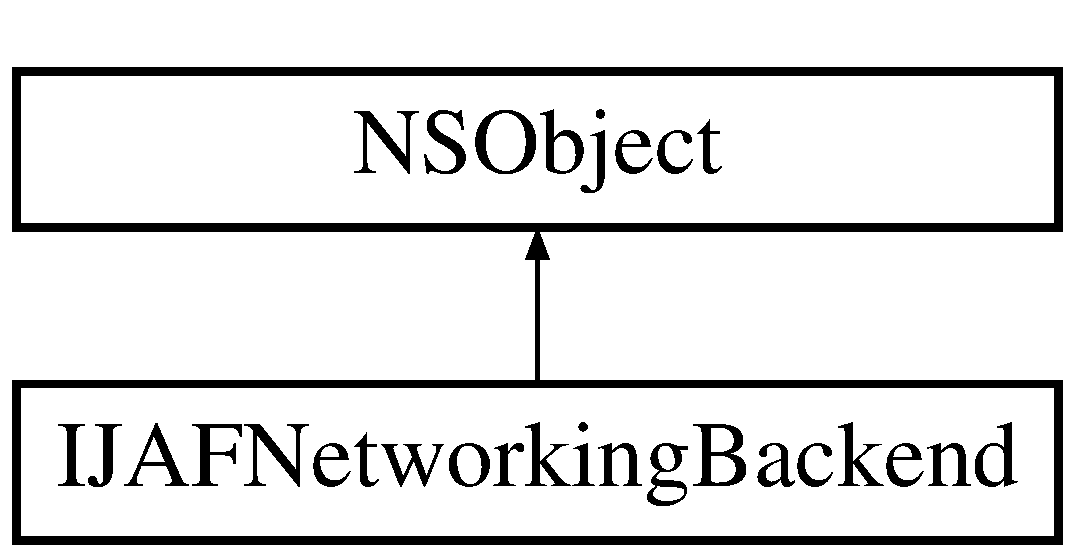
\includegraphics[height=2.000000cm]{interface_i_j_a_f_networking_backend}
\end{center}
\end{figure}
\subsection*{Instance Methods}
\begin{DoxyCompactItemize}
\item 
(void) -\/ \hyperlink{interface_i_j_a_f_networking_backend_a625df20d6ea6e780aafb7b438f66efad}{queue\+Request\+:success\+:failure\+:}
\begin{DoxyCompactList}\small\item\em This method add a request to a queue. \end{DoxyCompactList}\end{DoxyCompactItemize}
\subsection*{Properties}
\begin{DoxyCompactItemize}
\item 
N\+S\+Operation\+Queue $\ast$ \hyperlink{interface_i_j_a_f_networking_backend_ac2f0b3315f3a4761b445c5a822dd84c4}{operations\+Queue}
\end{DoxyCompactItemize}


\subsection{Method Documentation}
\hypertarget{interface_i_j_a_f_networking_backend_a625df20d6ea6e780aafb7b438f66efad}{\index{I\+J\+A\+F\+Networking\+Backend@{I\+J\+A\+F\+Networking\+Backend}!queue\+Request\+:success\+:failure\+:@{queue\+Request\+:success\+:failure\+:}}
\index{queue\+Request\+:success\+:failure\+:@{queue\+Request\+:success\+:failure\+:}!I\+J\+A\+F\+Networking\+Backend@{I\+J\+A\+F\+Networking\+Backend}}
\subsubsection[{queue\+Request\+:success\+:failure\+:}]{\setlength{\rightskip}{0pt plus 5cm}-\/ (void) queue\+Request\+: 
\begin{DoxyParamCaption}
\item[{(N\+S\+U\+R\+L\+Request $\ast$)}]{request}
\item[{success:(void($^\wedge$)(N\+S\+Operation $\ast$operation, id response\+Object))}]{success}
\item[{failure:(void($^\wedge$)({\bf I\+J\+Error} $\ast$error))}]{failure}
\end{DoxyParamCaption}
}}\label{interface_i_j_a_f_networking_backend_a625df20d6ea6e780aafb7b438f66efad}


This method add a request to a queue. 

This will add a request to a queue so you can stop all operations in case you don't need them anymore. In case you need to implement a not-\/contemplated method in your repositories you'll need to send your request here. Other way you won't never use it. 

\subsection{Property Documentation}
\hypertarget{interface_i_j_a_f_networking_backend_ac2f0b3315f3a4761b445c5a822dd84c4}{\index{I\+J\+A\+F\+Networking\+Backend@{I\+J\+A\+F\+Networking\+Backend}!operations\+Queue@{operations\+Queue}}
\index{operations\+Queue@{operations\+Queue}!I\+J\+A\+F\+Networking\+Backend@{I\+J\+A\+F\+Networking\+Backend}}
\subsubsection[{operations\+Queue}]{\setlength{\rightskip}{0pt plus 5cm}-\/ (N\+S\+Operation\+Queue$\ast$) operations\+Queue\hspace{0.3cm}{\ttfamily [read]}, {\ttfamily [write]}, {\ttfamily [atomic]}, {\ttfamily [strong]}}}\label{interface_i_j_a_f_networking_backend_ac2f0b3315f3a4761b445c5a822dd84c4}
The queue that handles the N\+S\+Operations 

The documentation for this class was generated from the following file\+:\begin{DoxyCompactItemize}
\item 
I\+K\+Jayma/\hyperlink{_i_j_a_f_networking_backend_8h}{I\+J\+A\+F\+Networking\+Backend.\+h}\end{DoxyCompactItemize}

\hypertarget{interface_i_j_error}{\section{I\+J\+Error Class Reference}
\label{interface_i_j_error}\index{I\+J\+Error@{I\+J\+Error}}
}


{\ttfamily \#import $<$I\+J\+Error.\+h$>$}

Inheritance diagram for I\+J\+Error\+:\begin{figure}[H]
\begin{center}
\leavevmode
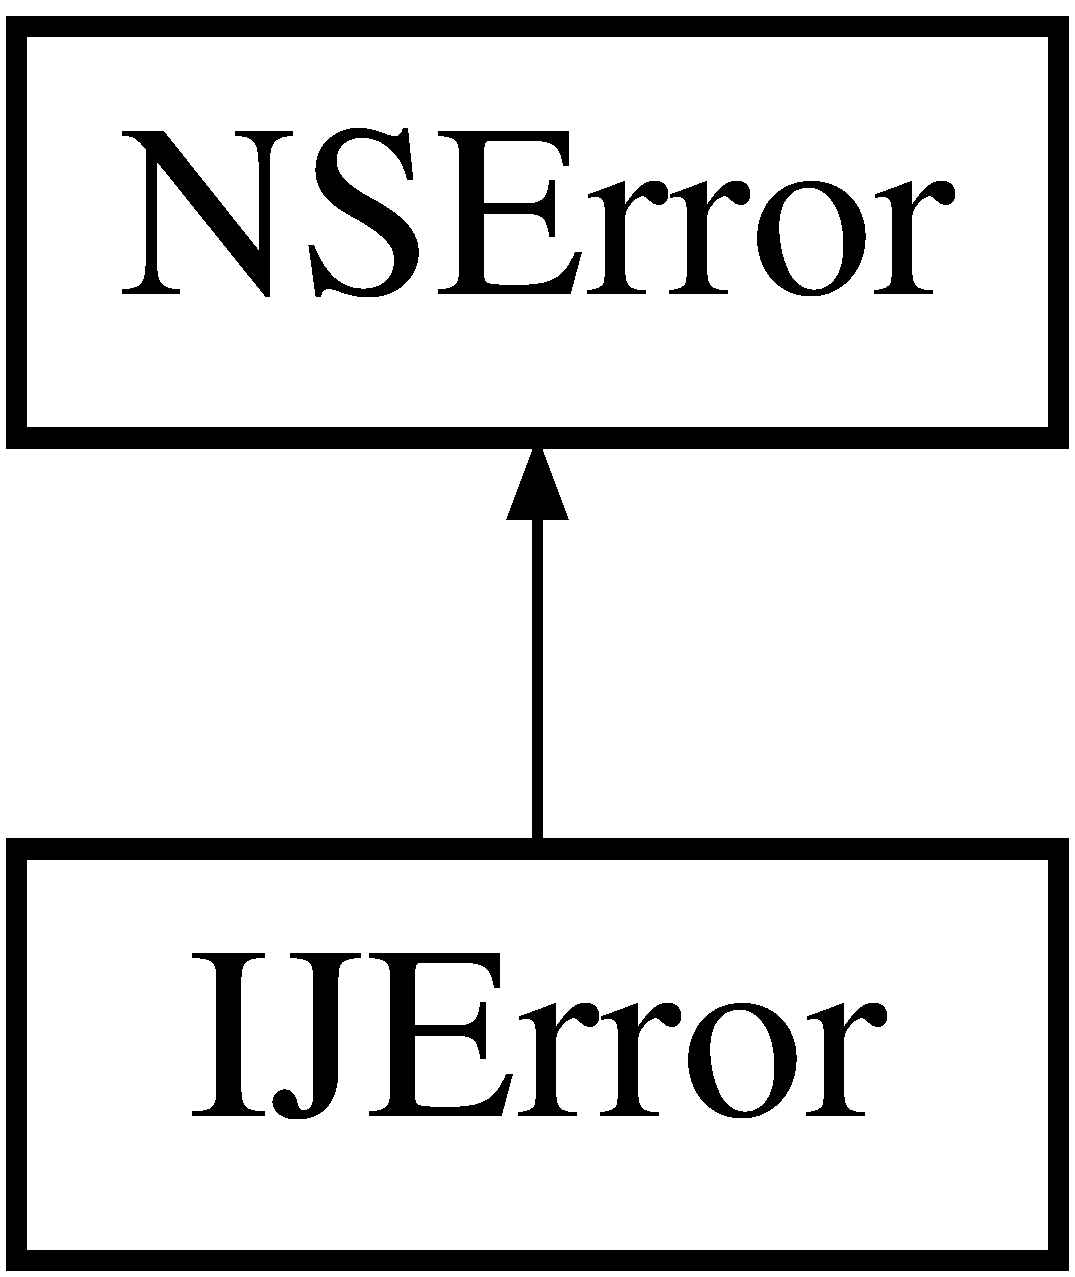
\includegraphics[height=2.000000cm]{interface_i_j_error}
\end{center}
\end{figure}
\subsection*{Instance Methods}
\begin{DoxyCompactItemize}
\item 
(id) -\/ \hyperlink{interface_i_j_error_a5629f8ba684d889b94903853ddeb53fa}{init\+With\+Response\+:response\+Object\+:and\+Error\+:}
\end{DoxyCompactItemize}
\subsection*{Properties}
\begin{DoxyCompactItemize}
\item 
N\+S\+H\+T\+T\+P\+U\+R\+L\+Response $\ast$ \hyperlink{interface_i_j_error_a44cfbf6891e5368a83d81407ac05ba4d}{response}
\item 
id \hyperlink{interface_i_j_error_ad9bbe1ee541238cfc14a42eb592260c6}{response\+Object}
\item 
N\+S\+Error $\ast$ \hyperlink{interface_i_j_error_a3ece78b392ee71d2f358312bff1bb75a}{internal\+Error}
\end{DoxyCompactItemize}


\subsection{Method Documentation}
\hypertarget{interface_i_j_error_a5629f8ba684d889b94903853ddeb53fa}{\index{I\+J\+Error@{I\+J\+Error}!init\+With\+Response\+:response\+Object\+:and\+Error\+:@{init\+With\+Response\+:response\+Object\+:and\+Error\+:}}
\index{init\+With\+Response\+:response\+Object\+:and\+Error\+:@{init\+With\+Response\+:response\+Object\+:and\+Error\+:}!I\+J\+Error@{I\+J\+Error}}
\subsubsection[{init\+With\+Response\+:response\+Object\+:and\+Error\+:}]{\setlength{\rightskip}{0pt plus 5cm}-\/ (id) init\+With\+Response\+: 
\begin{DoxyParamCaption}
\item[{(N\+S\+H\+T\+T\+P\+U\+R\+L\+Response $\ast$)}]{response}
\item[{responseObject:(id)}]{response\+Object}
\item[{andError:(N\+S\+Error $\ast$)}]{error}
\end{DoxyParamCaption}
}}\label{interface_i_j_error_a5629f8ba684d889b94903853ddeb53fa}
Assign the basic properties for an \hyperlink{interface_i_j_error}{I\+J\+Error} 

\subsection{Property Documentation}
\hypertarget{interface_i_j_error_a3ece78b392ee71d2f358312bff1bb75a}{\index{I\+J\+Error@{I\+J\+Error}!internal\+Error@{internal\+Error}}
\index{internal\+Error@{internal\+Error}!I\+J\+Error@{I\+J\+Error}}
\subsubsection[{internal\+Error}]{\setlength{\rightskip}{0pt plus 5cm}-\/ (N\+S\+Error$\ast$) internal\+Error\hspace{0.3cm}{\ttfamily [read]}, {\ttfamily [write]}, {\ttfamily [nonatomic]}, {\ttfamily [strong]}}}\label{interface_i_j_error_a3ece78b392ee71d2f358312bff1bb75a}
The N\+S\+Error retrieved by A\+F\+Networking. \hypertarget{interface_i_j_error_a44cfbf6891e5368a83d81407ac05ba4d}{\index{I\+J\+Error@{I\+J\+Error}!response@{response}}
\index{response@{response}!I\+J\+Error@{I\+J\+Error}}
\subsubsection[{response}]{\setlength{\rightskip}{0pt plus 5cm}-\/ (N\+S\+H\+T\+T\+P\+U\+R\+L\+Response$\ast$) response\hspace{0.3cm}{\ttfamily [read]}, {\ttfamily [write]}, {\ttfamily [nonatomic]}, {\ttfamily [strong]}}}\label{interface_i_j_error_a44cfbf6891e5368a83d81407ac05ba4d}
The N\+S\+H\+T\+T\+P\+U\+R\+L\+Response from the server. \hypertarget{interface_i_j_error_ad9bbe1ee541238cfc14a42eb592260c6}{\index{I\+J\+Error@{I\+J\+Error}!response\+Object@{response\+Object}}
\index{response\+Object@{response\+Object}!I\+J\+Error@{I\+J\+Error}}
\subsubsection[{response\+Object}]{\setlength{\rightskip}{0pt plus 5cm}-\/ (id) response\+Object\hspace{0.3cm}{\ttfamily [read]}, {\ttfamily [write]}, {\ttfamily [nonatomic]}, {\ttfamily [strong]}}}\label{interface_i_j_error_ad9bbe1ee541238cfc14a42eb592260c6}
The response object created by A\+F\+Networking. 

The documentation for this class was generated from the following file\+:\begin{DoxyCompactItemize}
\item 
I\+K\+Jayma/\hyperlink{_i_j_error_8h}{I\+J\+Error.\+h}\end{DoxyCompactItemize}

\chapter{File Documentation}
\hypertarget{_i_j_abstract_document_8h}{\section{I\+K\+Jayma/\+I\+J\+Abstract\+Document.h File Reference}
\label{_i_j_abstract_document_8h}\index{I\+K\+Jayma/\+I\+J\+Abstract\+Document.\+h@{I\+K\+Jayma/\+I\+J\+Abstract\+Document.\+h}}
}
{\ttfamily \#import $<$Foundation/\+Foundation.\+h$>$}\\*
\subsection*{Classes}
\begin{DoxyCompactItemize}
\item 
class \hyperlink{interface_i_j_abstract_document}{I\+J\+Abstract\+Document}
\end{DoxyCompactItemize}

\hypertarget{_i_j_abstract_repository_8h}{\section{I\+K\+Jayma/\+I\+J\+Abstract\+Repository.h File Reference}
\label{_i_j_abstract_repository_8h}\index{I\+K\+Jayma/\+I\+J\+Abstract\+Repository.\+h@{I\+K\+Jayma/\+I\+J\+Abstract\+Repository.\+h}}
}
{\ttfamily \#import $<$Foundation/\+Foundation.\+h$>$}\\*
{\ttfamily \#import \char`\"{}I\+J\+A\+F\+Networking\+Backend.\+h\char`\"{}}\\*
{\ttfamily \#import \char`\"{}I\+J\+Abstract\+Document.\+h\char`\"{}}\\*
{\ttfamily \#import \char`\"{}I\+J\+Error.\+h\char`\"{}}\\*
\subsection*{Classes}
\begin{DoxyCompactItemize}
\item 
class \hyperlink{interface_i_j_abstract_repository}{I\+J\+Abstract\+Repository}
\end{DoxyCompactItemize}

\hypertarget{_i_j_a_f_networking_backend_8h}{\section{I\+K\+Jayma/\+I\+J\+A\+F\+Networking\+Backend.h File Reference}
\label{_i_j_a_f_networking_backend_8h}\index{I\+K\+Jayma/\+I\+J\+A\+F\+Networking\+Backend.\+h@{I\+K\+Jayma/\+I\+J\+A\+F\+Networking\+Backend.\+h}}
}
{\ttfamily \#import $<$Foundation/\+Foundation.\+h$>$}\\*
{\ttfamily \#import $<$A\+F\+Networking/\+A\+F\+Networking.\+h$>$}\\*
{\ttfamily \#import \char`\"{}I\+J\+Error.\+h\char`\"{}}\\*
\subsection*{Classes}
\begin{DoxyCompactItemize}
\item 
class \hyperlink{interface_i_j_a_f_networking_backend}{I\+J\+A\+F\+Networking\+Backend}
\end{DoxyCompactItemize}

\hypertarget{_i_j_error_8h}{\section{I\+K\+Jayma/\+I\+J\+Error.h File Reference}
\label{_i_j_error_8h}\index{I\+K\+Jayma/\+I\+J\+Error.\+h@{I\+K\+Jayma/\+I\+J\+Error.\+h}}
}
{\ttfamily \#import $<$Foundation/\+Foundation.\+h$>$}\\*
\subsection*{Classes}
\begin{DoxyCompactItemize}
\item 
class \hyperlink{interface_i_j_error}{I\+J\+Error}
\end{DoxyCompactItemize}

%--- End generated contents ---

% Index
\newpage
\phantomsection
\addcontentsline{toc}{chapter}{Index}
\printindex

\end{document}
